% Section 6 - MDSplus
% Roberto Masocco <roberto.masocco@uniroma2.it>
% Alessandro Tenaglia <alessandro.tenaglia@uniroma2.it>
% June 5, 2024

% ### MDSplus ###
\section{MDSplus}
\graphicspath{{figs/section6/}}

% --- MDSplus ---
\begin{frame}{MDSplus}
	\begin{columns}
		\column{.6\textwidth}
		\begin{itemize}
			\item \textbg{MDSplus} is a tool for data acquisition and storage;
			\item \textbg{MDSplus} stores data in a user-defined hierarchical structure, namely a tree;
			\item A tree is formed by nodes, each of which represents a data field;
			\item Experiments of the same type have the same tree structure and an incremental pulse number;
		\end{itemize}
		\column{.4\textwidth}
		\begin{figure}
			\centering
			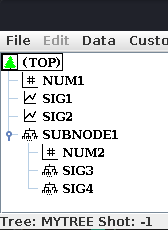
\includegraphics[scale=.5]{tree.png}
			\label{fig:tree}
			\caption{MDSplus tree}
		\end{figure}
	\end{columns}
\end{frame}
